%!TEX root = ../dokumentation.tex
\chapter{Grundlagen und Stand der Forschung}

%https://www-ai.cs.tu-dortmund.de/PublicPublicationFiles/bierwirth_2018a.pdf

\section{Implementierungsumgebung Jupyter}
Jupyter Notebooks ist eine von der non-profit Organisation Project Jupyter entwickelte Open-Source Lösung zur interaktiven Arbeit mit Dutzenden Programmiersprachen \cite{project_jupyter}. Der Name Jupyter leitet sich dabei von den drei primären Programmiersprachen Julia, Python und R ab. Jupyter Notebooks ist sprachunabhängig und unterstützt, unter Verwendung des IPython \gls{Kernel}, die Programmiersprachen Julia, R, Haskell, Ruby und Python \cite{jupyter_kernel}. Darüber hinaus werden unterschiedlichste Export Möglichkeiten wie \ac{HTML}, \ac{PDF} und \LaTeX \space unterstützt. Die in diesem Projekt verwendete Variante von Jupyter Notebooks ist Google Colab, eine speziell für die Python-Entwicklung entworfene Umgebung. Colab Notebooks führen Code auf Cloud-Servern aus und bieten somit unabhängige Vorteile gehosteter Hardware, wie \acp{GPU} und \acp{TPU} \cite{colab_notebooks}.

\section{Bildverarbeitungsalgorithmen mit OpenCV}

\section{Maschinelle Lernverfahren}

\subsection{Supervised Learning}

\subsection{Unsupervised Learning}

\subsection{Reinforcement Learning}

\section{Datenstromorientierte Programmierung mit TensorFlow}

\subsection{Künstliche neuronale Netze}

Die Ursprünge der künstlichen neuronalen Netze lassen sich auf \citeauthor{mcculloch_pitts} im Jahre \citeyear{mcculloch_pitts} zurückführen \cite{mcculloch_pitts}. Eine von Donald O. Hebb 1949 formulierte Lernregel stellt seither in ihrer allgemeinen Form die Grundlage der künstlichen neuronalen Lernverfahren dar \cite{Mainzer1997}.

Ein künstliches neuronales Netz besteht aus einer Eingabeschicht von Neuronen, $1..n$ versteckter Schichten und einer letzten Schicht von Ausgangsneuronen. Ein einzelnes Neuron nimmt überlicherweise mehrere Werte $x_{1},...,x_{n}$ und einen \gls{Bias}-Term $w_{0}$ als Eingabe und berechnet daraus die Ausgabe $y=h(z)$.

\begin{figure}[ht]
	\centering
	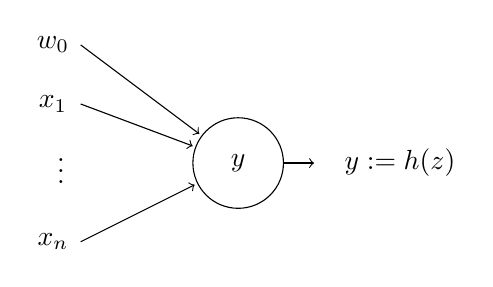
\begin{tikzpicture}[shorten >=1pt,->]
		\tikzstyle{unit}=[draw,shape=circle,minimum size=1.15cm]
 
		\node[unit](p) at (2,1){$y$};
		\node(dots) at (-0.25,1){\vdots};
 
		\draw (0,2.5) node[xshift=-10]{$w_0$} -- (p);
		\draw (0,1.75) node[xshift=-10]{$x_1$} --(p);
		\draw (0,0) node[xshift=-10]{$x_n$} -- (p);
		\draw (p) -- (3,1) node[xshift=30]{$y := h(z)$};
	\end{tikzpicture}
	\caption[Einzelnes Neuron mit dessen Komponenten]{Einzelnes Neuron mit dessen Eingangsvariablen. Die Aktivierungsfunktion ist beschrieben als $h$ und wird auf die tatsächlichen Eingabe $z$ angewandt. $x_1 ,..., x_n$ repräsentieren die Eingabe von anderen Neuronen innerhalb des Netzes. $w_0$ wird \gls{Bias} genannt und repräsentiert ein externes Gewicht \cite{stutz_neural_networks}.}
	\label{fig:processing-unit}
\end{figure}

Die Ausgabe $h_{i}$ des Neurons $i$ in der versteckten Schicht wird beschrieben durch

\begin{equation}
	h_{i} = \varphi(\sum_{j=1}^N{V_{ij}x_{j}+\theta_{i}^{hid}})
\end{equation}

wo $\varphi(\cdot)$ die Aktivierungsfunktion, $N$ die Anzahl der Eingangsneuronen, $V_{ij}$ die Gewichte, $x_{j}$ die Eingabe zum Neuron und $\theta_{i}^{hid}$ der Schwellenwertterm der versteckten Neuronen ist \cites[81-100]{Wang2003}[195-201]{Networks1995}. Die Intention der Aktivierungsfunktion $\varphi(\cdot)$ neben der Einführung von Nichtlinearität in das neuronale Netz ist, den Wert eines Neurons zu begrenzen, damit das neuronale Netz nicht durch divergierende Neuronen gelähmt wird. Eine gängige Aktivierungsfunktion ist die Sigmoid Funktion $\sigma(\cdot)$, wie definiert in \ref{eq:sigmoid}.

\begin{equation}\label{eq:sigmoid}
	\sigma(u) = \frac{1}{1 + e^{-u}}
\end{equation}


Weitere sigmoide Aktivierungsfunktionen sind der Arkustangens ($\arctan$) und Tangens Hyperbolikus ($\tanh$) \cite[195-201]{Networks1995}. Sie haben ein ähnliches Ansprechverhalten auf die Eingangswerte wie die Sigmoidfunktion, unterscheiden sich aber in den Ausgangsbereichen. 

\begin{figure}[htb]
\centering
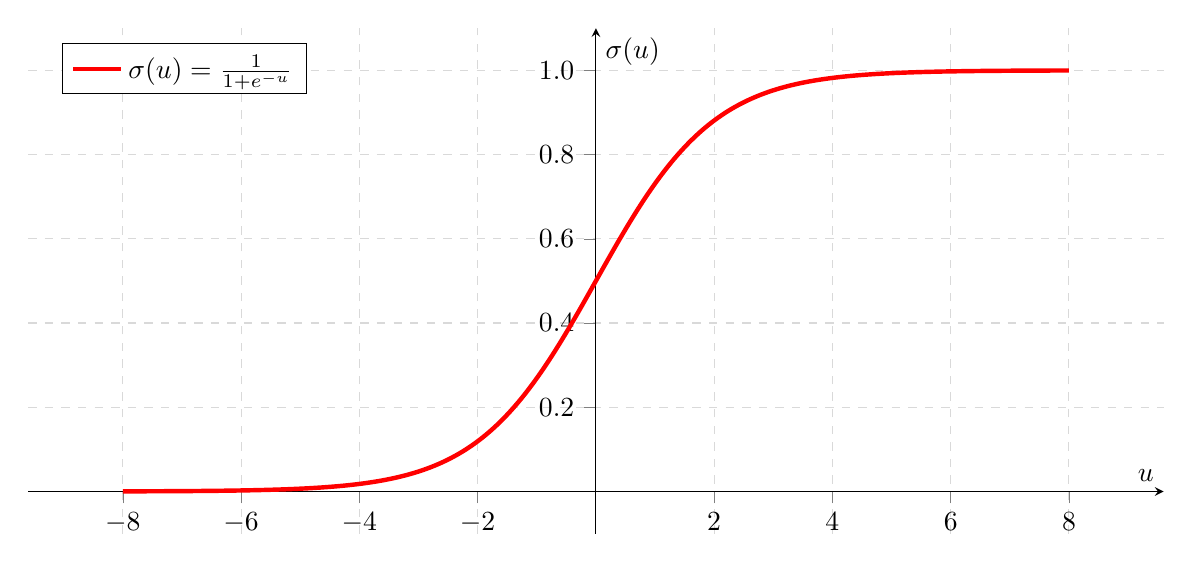
\begin{tikzpicture}\label{fig:sigmoid}
    \begin{axis}[
        legend pos=north west,
        axis x line=middle,
        axis y line=middle,
        y tick label style={/pgf/number format/fixed,
                            /pgf/number format/fixed zerofill,
                            /pgf/number format/precision=1},
        grid = major,
        width=16cm,
        height=8cm,
        grid style={dashed, gray!30},
        xmin=-8,     % start the diagram at this x-coordinate
        xmax= 8,     % end   the diagram at this x-coordinate
        ymin= 0,     % start the diagram at this y-coordinate
        ymax= 1,     % end   the diagram at this y-coordinate
        %axis background/.style={fill=white},
        xlabel=$u$,
        ylabel=$\sigma(u)$,
        tick align=outside,
        enlargelimits=true]
      % plot the stirling-formulae
      \addplot[domain=-8:8, red, ultra thick,samples=500] {1/(1+exp(-1*x))};
      \addlegendentry{$\sigma(u)=\frac{1}{1+e^{-u}}$}
    \end{axis}
\end{tikzpicture}
\caption{Darstellung der Sigmoid Aktivierungsfunktion}
\end{figure}

\subsection{Convolutional Neural Networks}

Seitdem \gls{AlexNet} im Jahre 2012 eine Auszeichnung beim jährlichen Wettbewerb der Benchmark-Datenbank ImageNet erzielte \cite{imagenet}, hat sich der Forschungsfokus auf das Themengebiet \emph{Deep Learning} zubewegt \cites{NIPS2012_c399862d, rastegari2016xnornet, russakovsky2015imagenet}. Zuvor waren \acp{SVM} der prävaliernde Ansatz zur Erkennung von Mustern.

\acp{CNN} werden seit 1995 in der digitalen Bildverarbeitung eingesetzt und sind fester Bestandteil des \emph{Deep Learnings}. Es werden Faltmatrizen der Größe 3x3, 5x5, 7x7 bzw. 9x9 eingesetzt, um Bereiche der Eingabematrix sukzessiv zu analysieren. Die dabei verwendeten \emph{convolutional operations} (Faltoperationen) erzeugen rezeptive Felder, die eine Merkmalskarte (\emph{feature map}) des \ac{CNN} generieren \cite{russakovsky2015imagenet}. Die rezeptiven Felder korrespondieren mit einer Region aus dem Originalbild \cite{Yan2020}. 
% Begin Figure CNN Matrix
\usetikzlibrary{matrix,positioning}
\begin{figure}[htb]
\centering
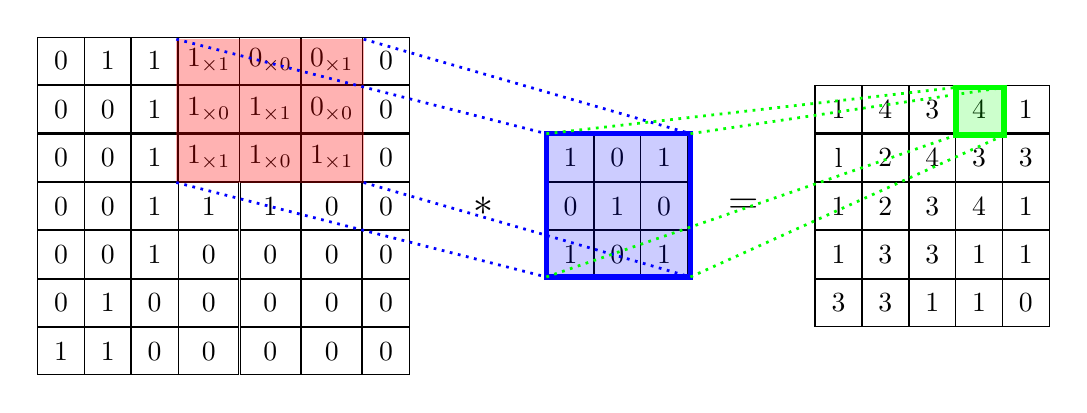
\begin{tikzpicture}[scale=1.0]

  \matrix [nodes=draw,column sep=-0.2mm, minimum size=6mm]
  {
    \node {0}; & \node{1}; & \node {1}; & \node{$1_{\times 1}$}; & \node{$0_{\times 0}$}; 
    & \node{$0_{\times 1}$}; & \node{0}; \\
    \node {0}; & \node{0}; & \node {1}; & \node{$1_{\times 0}$}; & \node{$1_{\times 1}$}; 
    & \node{$0_{\times 0}$}; & \node{0}; \\
    \node {0}; & \node{0}; & \node {1}; & \node{$1_{\times 1}$}; & \node{$1_{\times 0}$}; 
    & \node{$1_{\times 1}$}; & \node{0}; \\
    \node {0}; & \node{0}; & \node {1}; & \node{\, 1 \,}; & \node{\, 1 \, }; 
    & \node{\, 0 \,}; & \node{0}; \\
    \node {0}; & \node{0}; & \node {1}; & \node{\, 0 \, }; & \node{\, 0 \, }; 
    & \node{\, 0 \,}; & \node{0}; \\
    \node {0}; & \node{1}; & \node {0}; & \node{\, 0 \, }; & \node{\, 0 \, }; 
    & \node{\, 0 \,}; & \node{0}; \\
    \node {1}; & \node{1}; & \node {0}; & \node{\, 0 \,}; & \node{\, 0 \, }; 
    & \node{\, 0 \,}; & \node{0}; \\
  };


  % coordinates for coloring filter in array
  \coordinate (A) at (-0.6,0.3);
  \coordinate (B) at (1.78,0.3);
  \coordinate (C) at (1.78,2.12);
  \coordinate (D) at (-0.6,2.12);
  \fill[red, opacity=0.3] (A)--(B)--(C)--(D)--cycle;
  \begin{scope}[shift={(3.3,0)}]
    \node[] at (0,0) {\Large $\ast$};
  \end{scope}[shift={(2.5,0)}]

  \begin{scope}[shift={(5,0)}]

    %\matrix [matrix of math nodes,left delimiter={[},right
    %delimiter={]}]
    \matrix [nodes=draw,column sep=-0.2mm, minimum size=6mm]
    {
      \node{1};  & \node{0};   & \node{1};  \\
      \node{0};  & \node{1};   & \node{0};  \\
      \node{1}; & \node{0}; & \node{1}; \\
    };
    \coordinate (A1) at (-0.9,-0.9);
    \coordinate (B1) at (0.93,-0.9);
    \coordinate (C1) at (0.93,0.92);
    \coordinate (D1) at (-0.9,0.92);
    \fill[blue, opacity=0.2] (A1)--(B1)--(C1)--(D1)--cycle;
    \draw[blue, line width=2] (A1)--(B1)--(C1)--(D1)--cycle;
  \end{scope}

  \draw[dotted, line width=1, color=blue] (A)--(A1);
  \draw[dotted, line width=1, color=blue] (B)--(B1);
  \draw[dotted, line width=1, color=blue] (C)--(C1);
  \draw[dotted, line width=1, color=blue] (D)--(D1);

  \begin{scope}[shift={(6.6,0)}]
    \node[] at (0,0) {\Large $=$};
  \end{scope}[shift={(2.5,0)}]

  \begin{scope}[shift={(9,0)}]

    %\matrix [matrix of math nodes,left delimiter={[},right
    %delimiter={]}]
    \matrix [nodes=draw,column sep=-0.2mm, minimum size=6mm]
    {
      \node{1};  & \node{4};   & \node{3}; & \node{4}; & \node{1};  \\
      \node{l};  & \node{2};   & \node{4}; & \node{3}; & \node{3};  \\
      \node{1}; & \node{2}; & \node{3}; & \node{4} ; & \node{1};  \\
      \node{1}; & \node{3}; & \node{3}; & \node{1} ; & \node{1};  \\
      \node{3}; & \node{3}; & \node{1}; & \node{1} ; & \node{0};  \\
    };
    \coordinate (A2) at (0.3,0.9);
    \coordinate (B2) at (0.91,0.9);
    \coordinate (C2) at (0.91,1.507);
    \coordinate (D2) at (0.3,1.507);
    \fill[green, opacity=0.2] (A2)--(B2)--(C2)--(D2)--cycle;
    \draw[green, line width=2] (A2)--(B2)--(C2)--(D2)--cycle;
  \end{scope}

  \draw[dotted, line width=1, color=green] (A1)--(A2);
  \draw[dotted, line width=1, color=green] (B1)--(B2);
  \draw[dotted, line width=1, color=green] (C1)--(C2);
  \draw[dotted, line width=1, color=green] (D1)--(D2);
\end{tikzpicture}
\caption{Erzeugen einer Merkmalskarte durch schrittweise Faltung}
\end{figure}


In der Mathematik wird die Faltung als eine Operation auf zwei Funktionen $f,g$ beschrieben, die eine dritte Funktion $f * g$ erzeugt. Die dritte Funktion beschreibt, wie die Form von $f$ durch $g$ verändert oder gefiltert wird. Für eine Position $ z_{ i,j } $ in der Ausgabe gilt

\begin{equation}
	z_{i,j}=b+\sum_{u=0}^{f_{h}-1}\sum_{v=0}^{f_{w}-1}{x_{i+u,j+v}\cdot w_{u,v}}
\end{equation}

worin $z_{i,j}$ die Position innerhalb der Matrix $z$ beschreibt und $b$ der \gls{Bias} ist. Betrachtet man nun die Position $z_{i,j}$ in der Ausgabe eines Layers gilt 

\begin{equation}
	z_{i,j}=b+\sum_{u=0}^{f_{h}-1}\sum_{v=0}^{f_{w}-1}{x_{i',j'}\cdot w_{u,v}}\text{  \space\space\space    } \begin{cases}
	i' = i \cdot s_{h} + u \\ j' = j \cdot s_{w} + v 
\end{cases}
\end{equation}

Die darauffolgende \emph{Volume Convolution} erweitert die Gleichung um einen Parameter $k$ , der die Anzahl der Farbräume in die Gleichung einbezieht. Es gilt
	
\begin{equation}
	z_{i,j,k'}=b_{k'}+\sum_{c=1}^k{}\sum_{u=0}^{f_{h}-1}\sum_{v=0}^{f_{w}-1}{x_{i',j',c}\cdot w_{u,v,c,k'}}\text{  \space\space\space    } \begin{cases}
	i' = i \cdot s_{h} + u \\ j' = j \cdot s_{w} + v 
\end{cases}
\end{equation}
Die Anzahl der Parameter eines \ac{CNN} ist unabhängig von der Eingabe, jedoch abhängig von der Größe des Filters. Allgemein gilt daher 

\begin{equation}
	\text{\#{ }Params}_{conv} = (f_{w} \cdot f_{h} \cdot k^{l-1} + 1) \cdot k^l
\end{equation}








\section{Deep Learning mit Keras}

\section{Verwandte Arbeiten}
